\documentclass{article}

\usepackage[utf8]{inputenc}
\usepackage{amsfonts}
\usepackage{amsmath}
\usepackage{amsthm}
\usepackage{blindtext}
\usepackage{graphicx}
\usepackage{natbib}
\usepackage{amssymb}

\newtheorem{theorem}{Theorem}
\newtheorem{lemma}{Lemma}
\newtheorem{corollary}{Corollary}
\newtheorem{conjecture}{Conjecture}
\newtheorem{proposition}{Proposition}
\theoremstyle{definition}
\newtheorem{definition}{Definition}
\newtheorem{remark}{Remark}


\title{Hammond's Project and Simple Random Graphs}
\author{by Alan Hammond, Milo Moses, Samuel Packman, Emma Lynch, Benjamin Lemkin}
\begin{document}
\maketitle

\newcommand{\lcm}{\mathrm{lcm}}


\tableofcontents
\newcommand{\R}{\mathbb{R}}
\newcommand{\Z}{\mathbb{Z}}
\newcommand{\N}{\mathbb{N}}
\newcommand{\C}{\mathbb{C}}
\newcommand{\class}{\mathcal{C}}
\newcommand{\E}{\mathbb{E}_{B}}
\newcommand{\Esup}{\mathbb{E}^{\mathrm{sup}}_{n\in\mathbb{N}}}
\newcommand{\rad}{\mathrm{rad}}

\addcontentsline{toc}{section}{}

\section{Introduction}

In this project, the authors seek to understand the behavior of Simple Random Bridge (SRBs), and more specfically how they behave under addition. An SRG of size $N$ is a function $B:\Z/N\Z\to\Z$ such that $B(0)=0$ and $B(x+1)-B(x)=\pm 1$ for all $x\in \Z/N\Z$.

\begin{figure}[h]
\caption{An Example of a SRB}
\centering
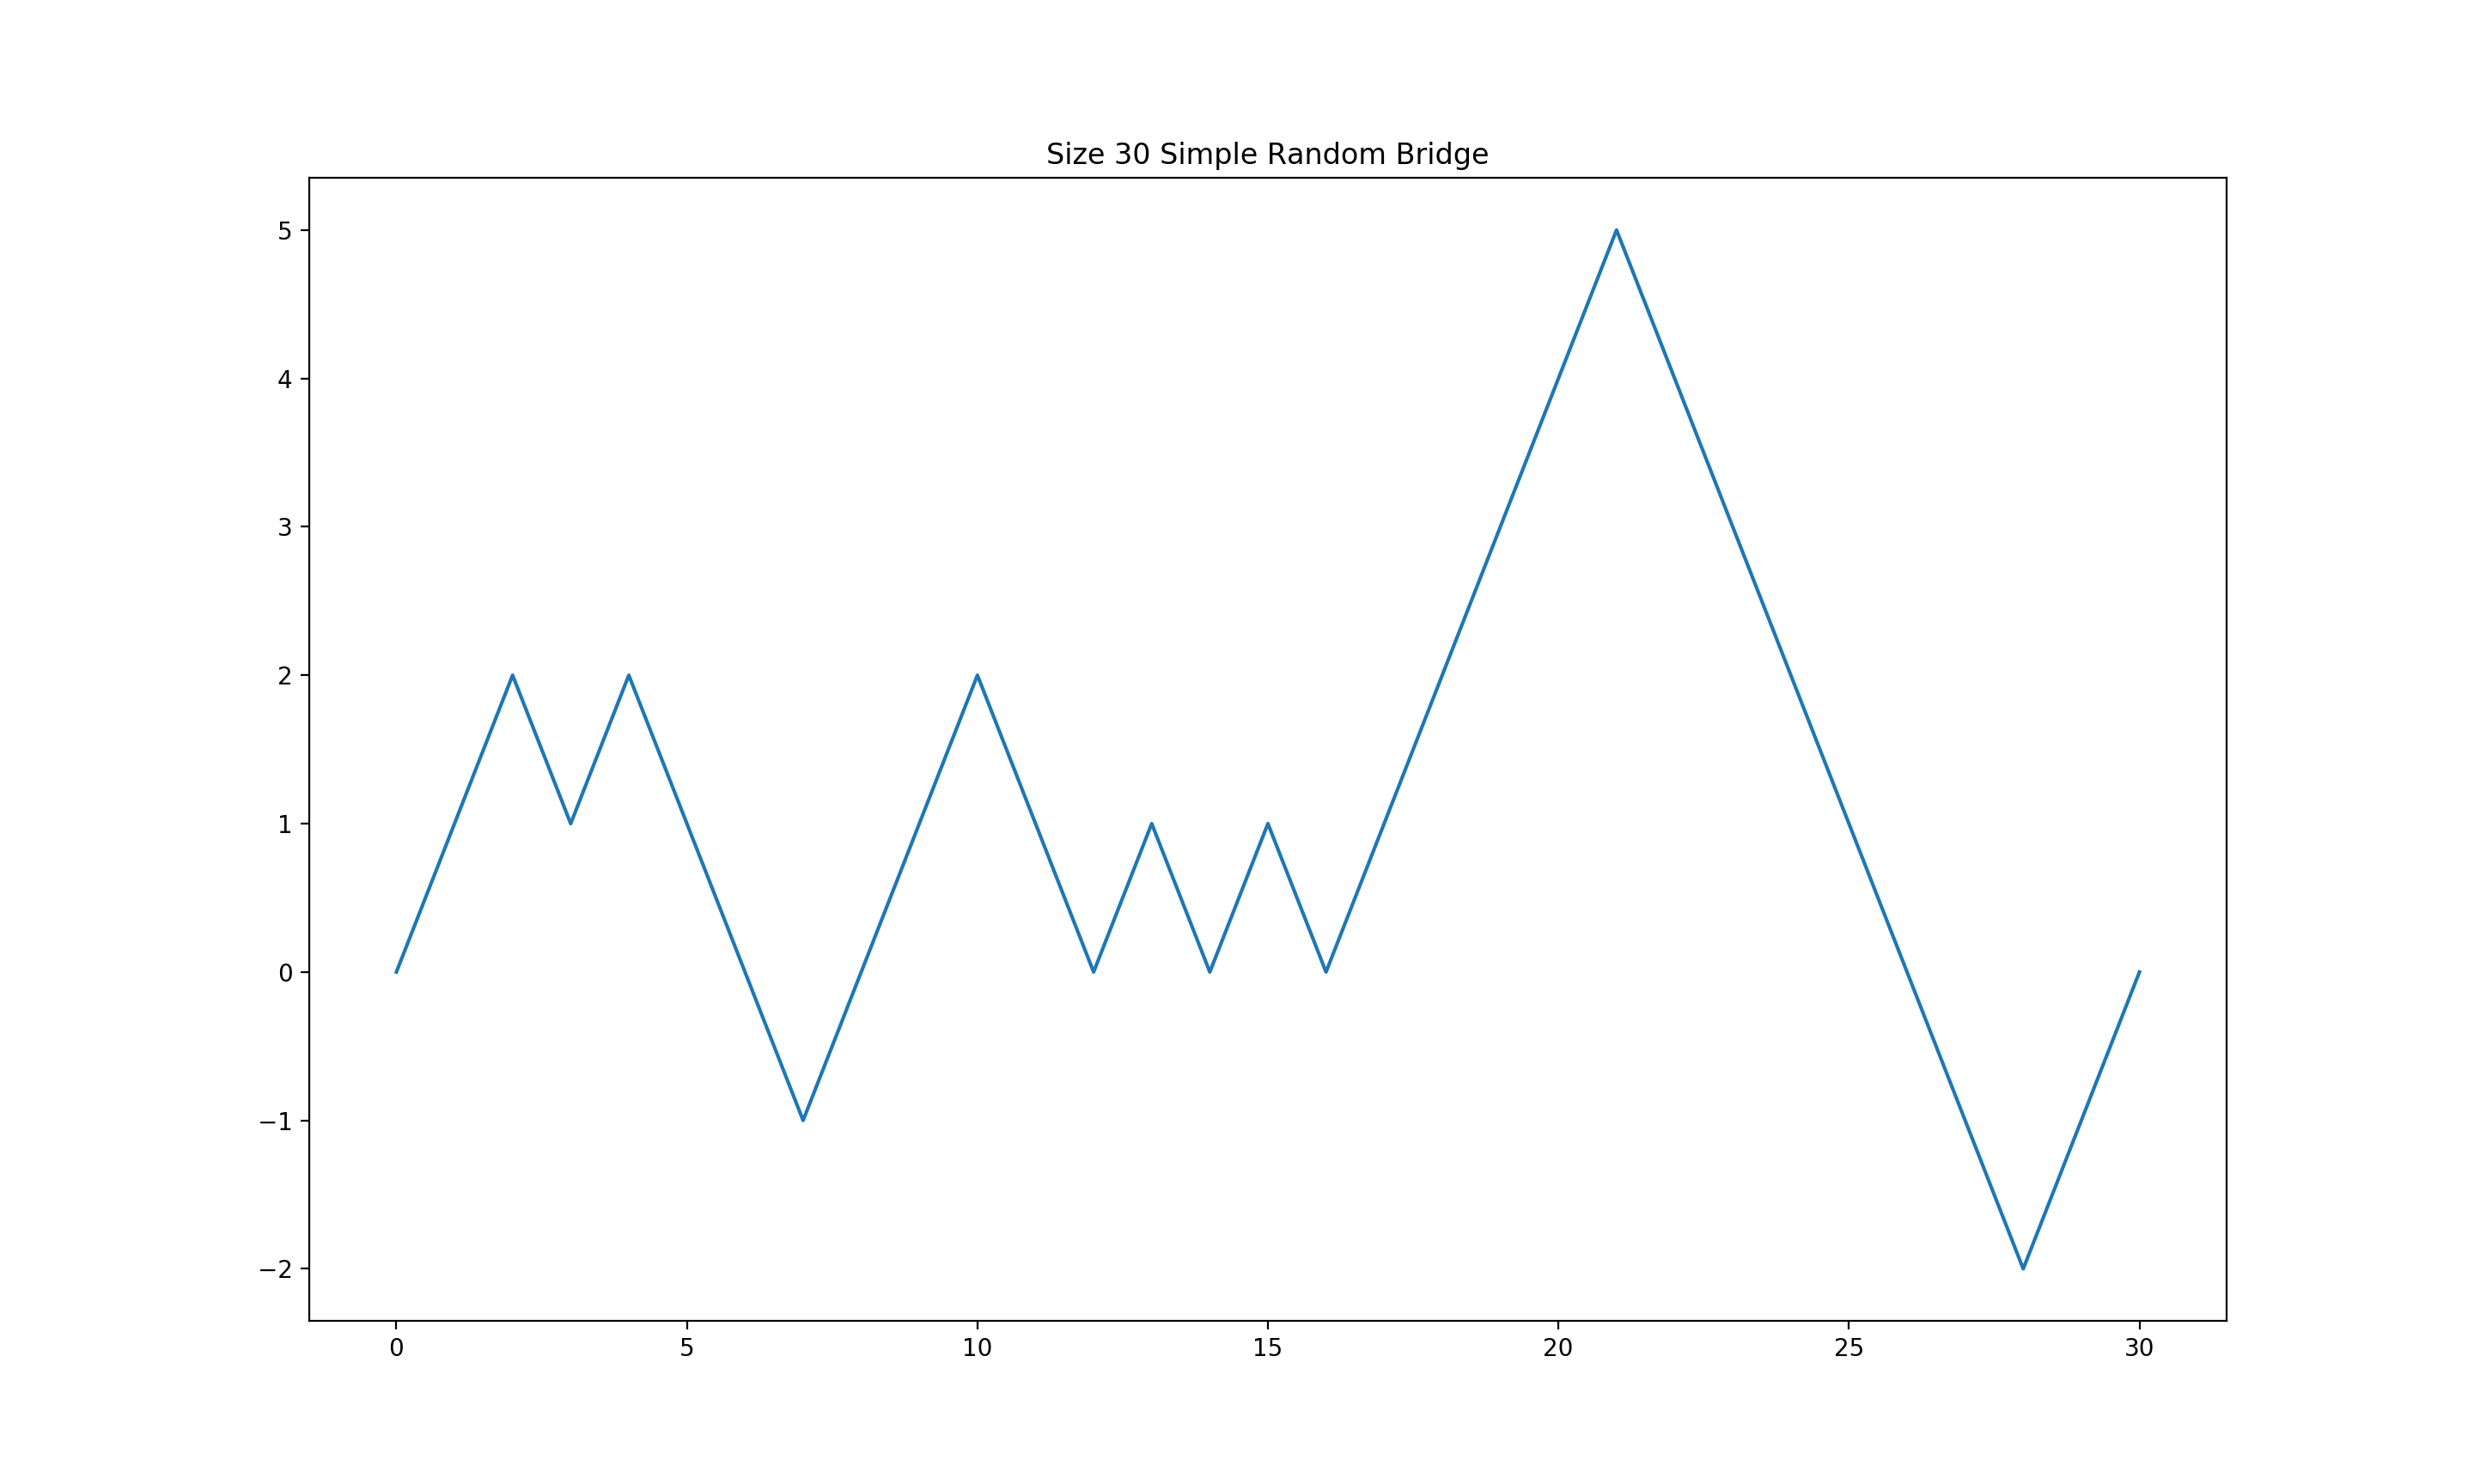
\includegraphics[width=\textwidth]{Figure_1}
\end{figure}

We say that a value $i\in \Z/N\Z$ is $\mathit{down}$ in $B$ if $B(i)<\min(B(i-1),B(i+1))$.

If $B_1$ and $B_2$ are size $N$ bridges, then we say that the $\mathit{minimal \,\,points}$ of $B_1$ under $B_2$ are those values $i\in \Z/N\Z$ such that $B_1(i)-B_2(i)=\min_{j}\left(B_1(j)-B_2(j)\right)$. If $0$ is not minimal then we define the $\mathit{addition}$ of $B_2$ to $B_1$ as

\begin{equation*}
\tilde{B_1}(i)=\begin{cases} B_1(i)+2 & i \,\,\mathrm{minimal\,\, under\,\,}B_2 \\
B_1(i)& \mathrm{otherwise}
\end{cases}
\end{equation*}

If $0$ is minimal, then we define

\begin{equation*}
\tilde{B_1}(i)=\begin{cases} B_1(i)-2 & i \,\,\mathrm{not\,\,minimal\,\,under\,\,}B_2 \\
B_1(i)& \mathrm{otherwise}
\end{cases}
\end{equation*}

It is clear that in both cases $\tilde{B_1}$ is once again an SRB. We note the interpretation of addition as putting $B_2$ below $B_1$ (as graphs) and sliding $B_2$ up until it just touches $B_1$, at which point every down intersection point is flipped up. In the case that $0$ is minimal, everything is then rescaled down so that $\tilde{B_1}(0)=0$.

The main interest of this paper is the result of repeated addition of a template bridge $B_1$ to random trial bridges, where in this context random means taken uniformly over the (finite) space of SRBs of size $N$.

\begin{figure}[h!]
\caption{An SRB after repeated addition}
\centering
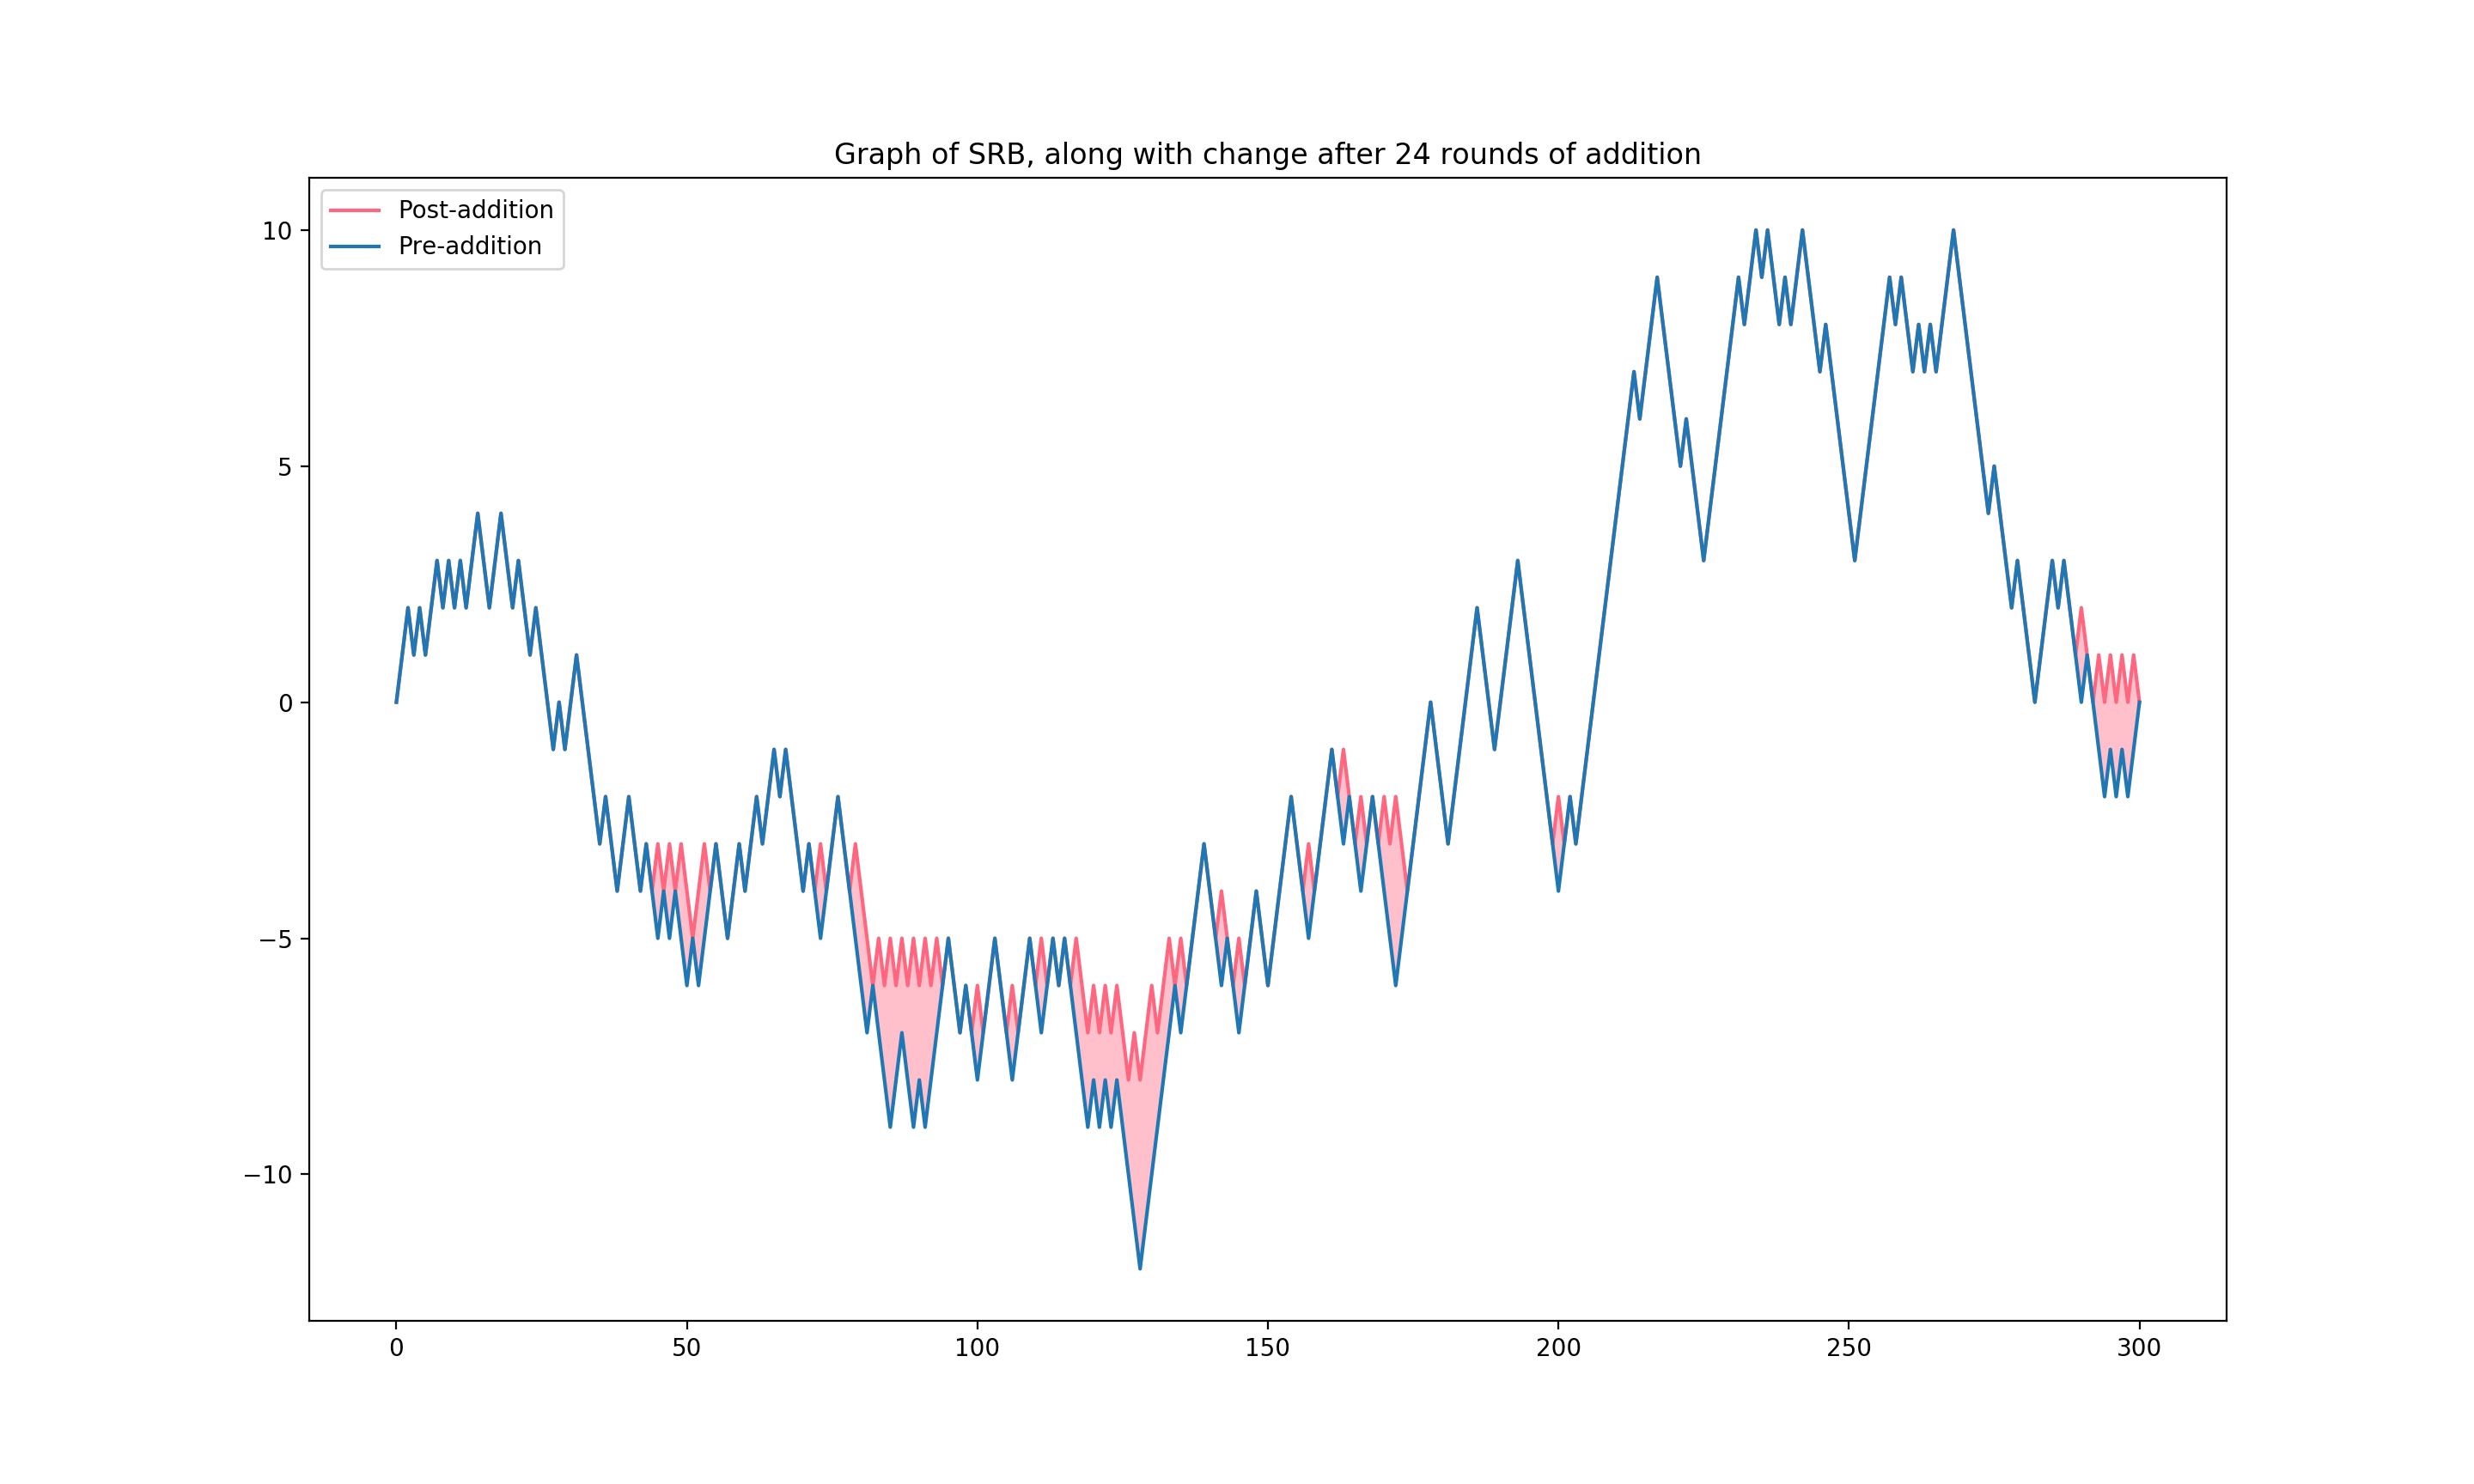
\includegraphics[width=\textwidth]{Figure_2}
\end{figure}

\section{Flattening effect of repeated addition}

One natural phenominon to observe the probability that any given SRB appears after large rounds of repeated addition. A sampling of 100 random SRBs of size 176 before and after 10,000 rounds of repeated addition by random SRBs is shown in Figure 3.

\begin{figure}[h!]
\caption{An SRB after repeated addition}
\centering
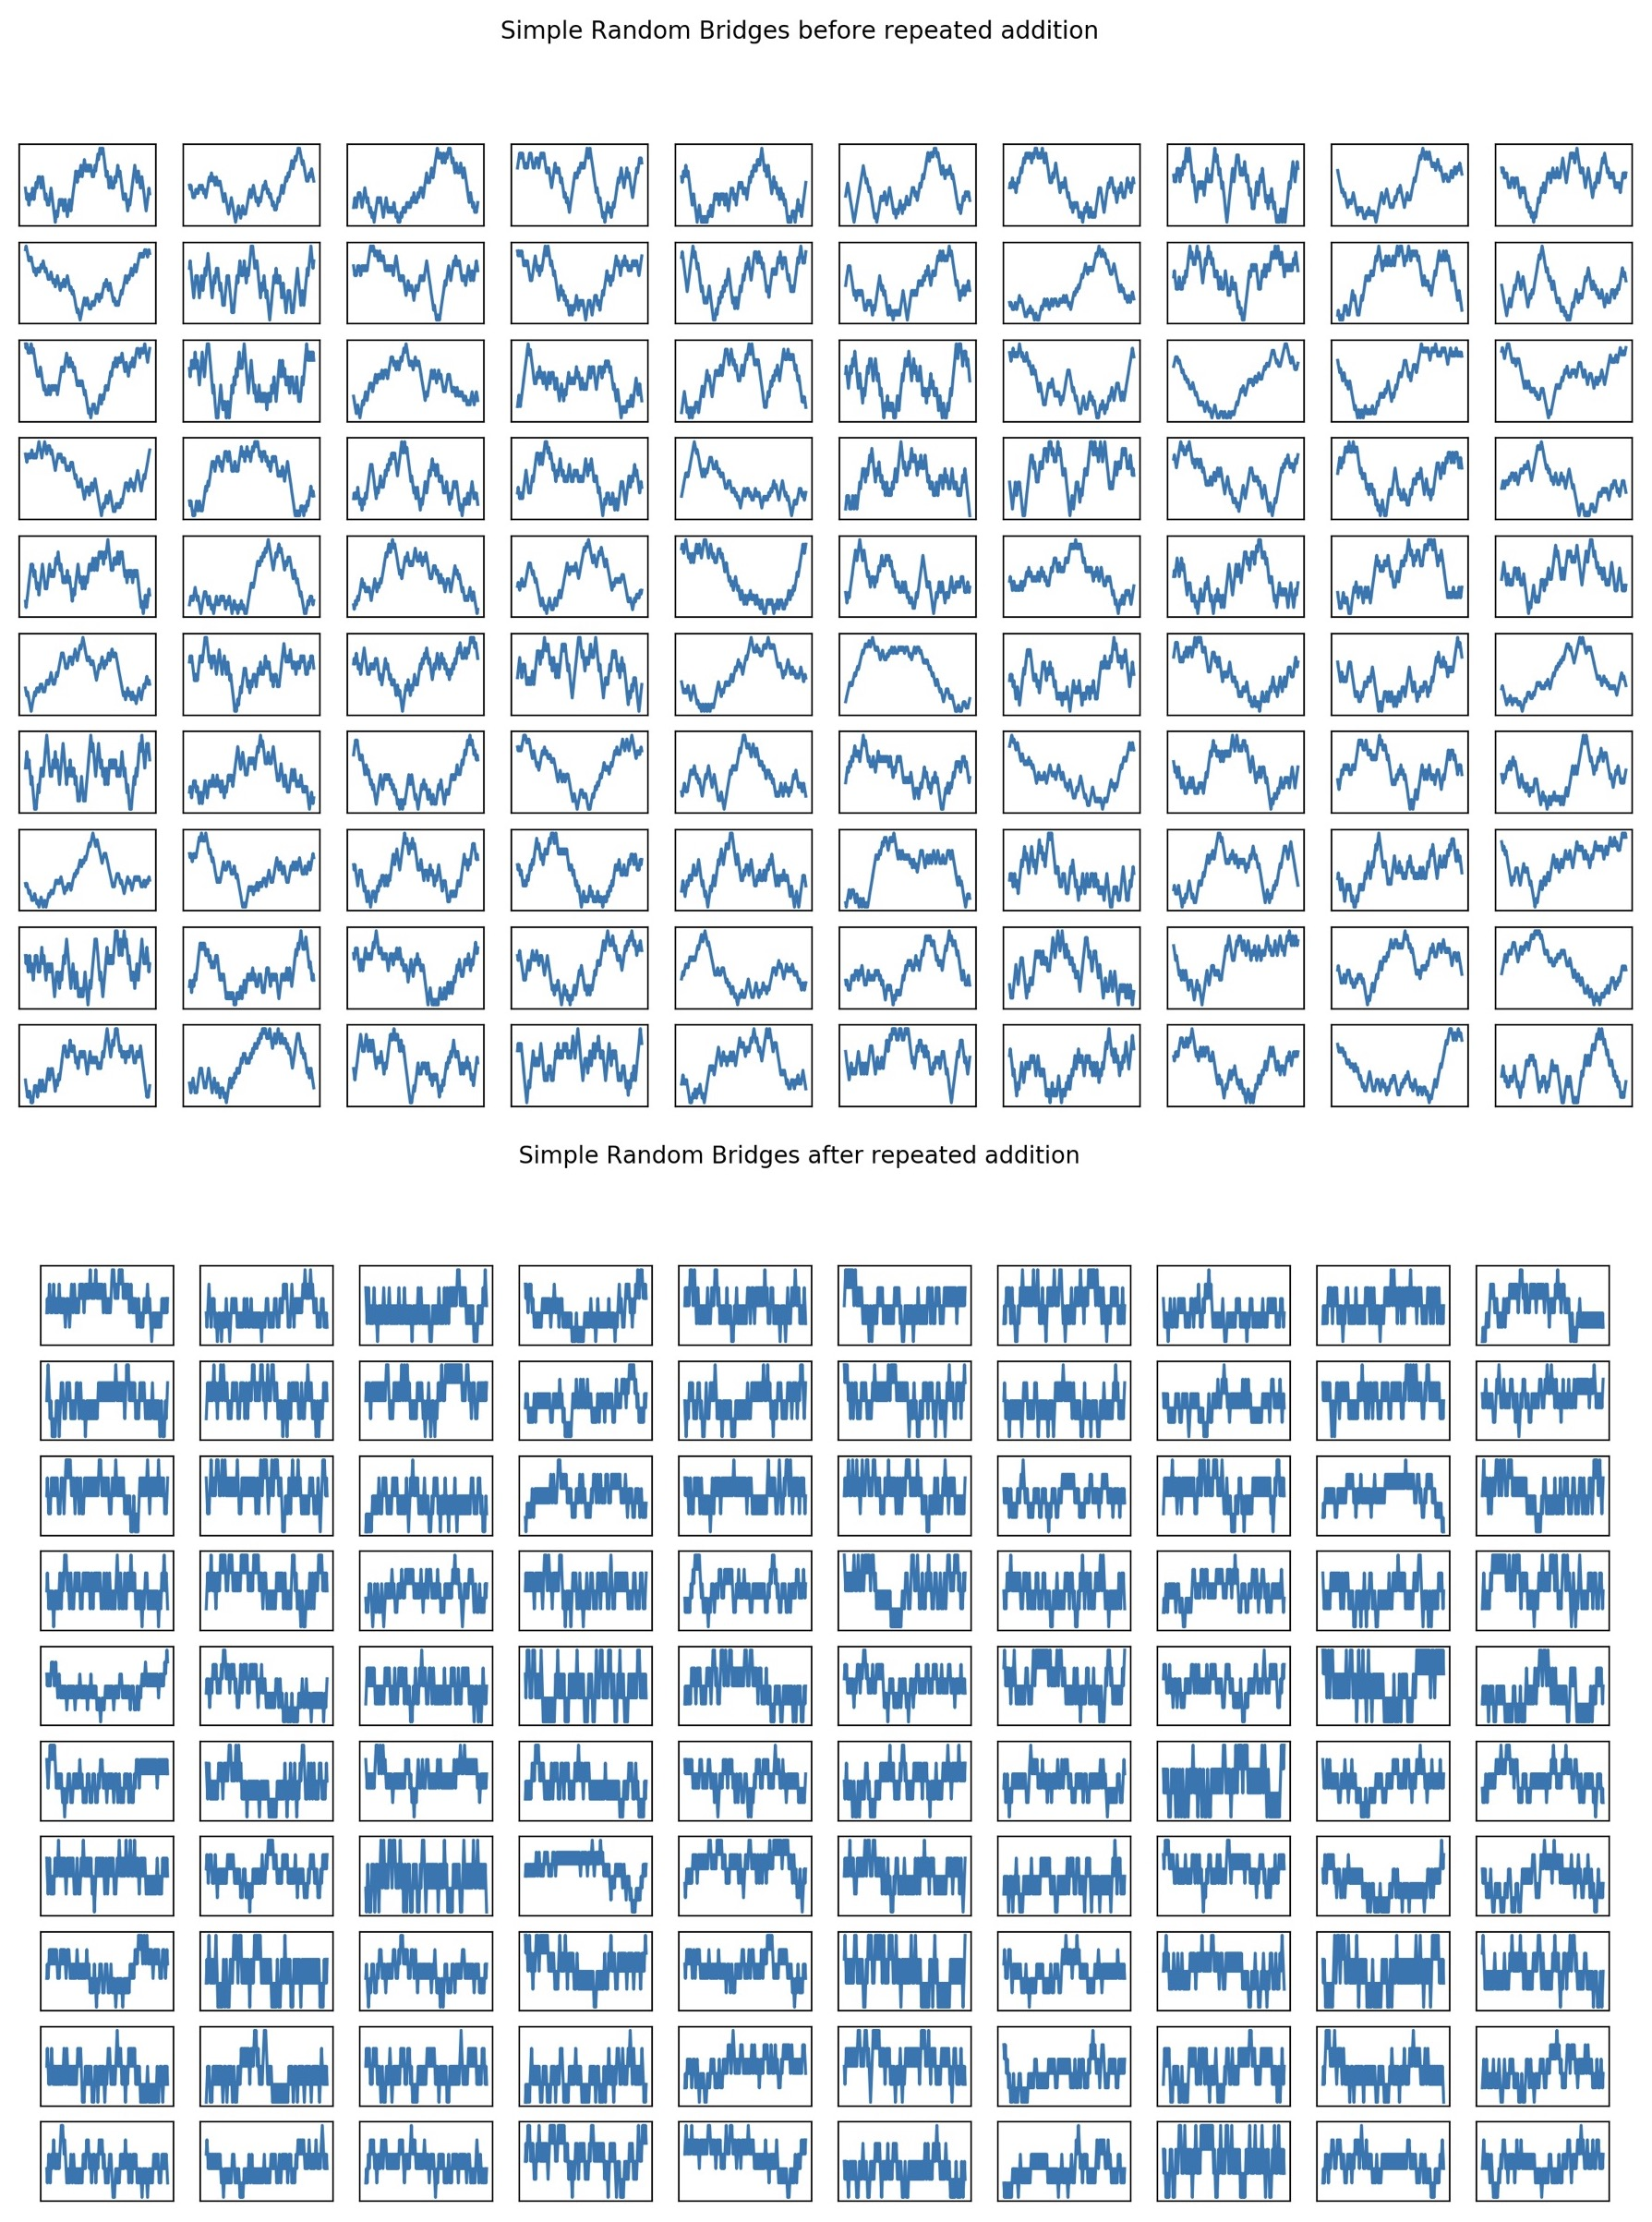
\includegraphics[width=.75\textwidth]{Figure_3}
\end{figure}

Note the the thick bars in the "after repeated addition" group. These show that the values of $B$ are distributed across a very small image. This can be measured in the quantity $s(N):=\E\left[\max_{i}|B(i)|\right]$ where the expected value is taken over all bridges $B$ of size $N$, weigthed according to how likely they are to appear after an arbitrarily large amount of flips from an arbitrary starting bridge. This example demonstrates the fact that, numerically, $s(176)$ seems to be about $2.8$.

Figure 4 shows how the numerically approximated quanity $s(N)$ changes as $N$ varies. Due to the extremely sharp fit of the superimposed logarithm, the following conjecture is clearly motivated:

\begin{conjecture} The value $\lim_{N\to\infty}\frac{s(N)}{\ln(N)}$ converges to a value $0<c<\infty$.
\end{conjecture}

\begin{figure}[h!]
\caption{s(N) versus $N$}
\centering
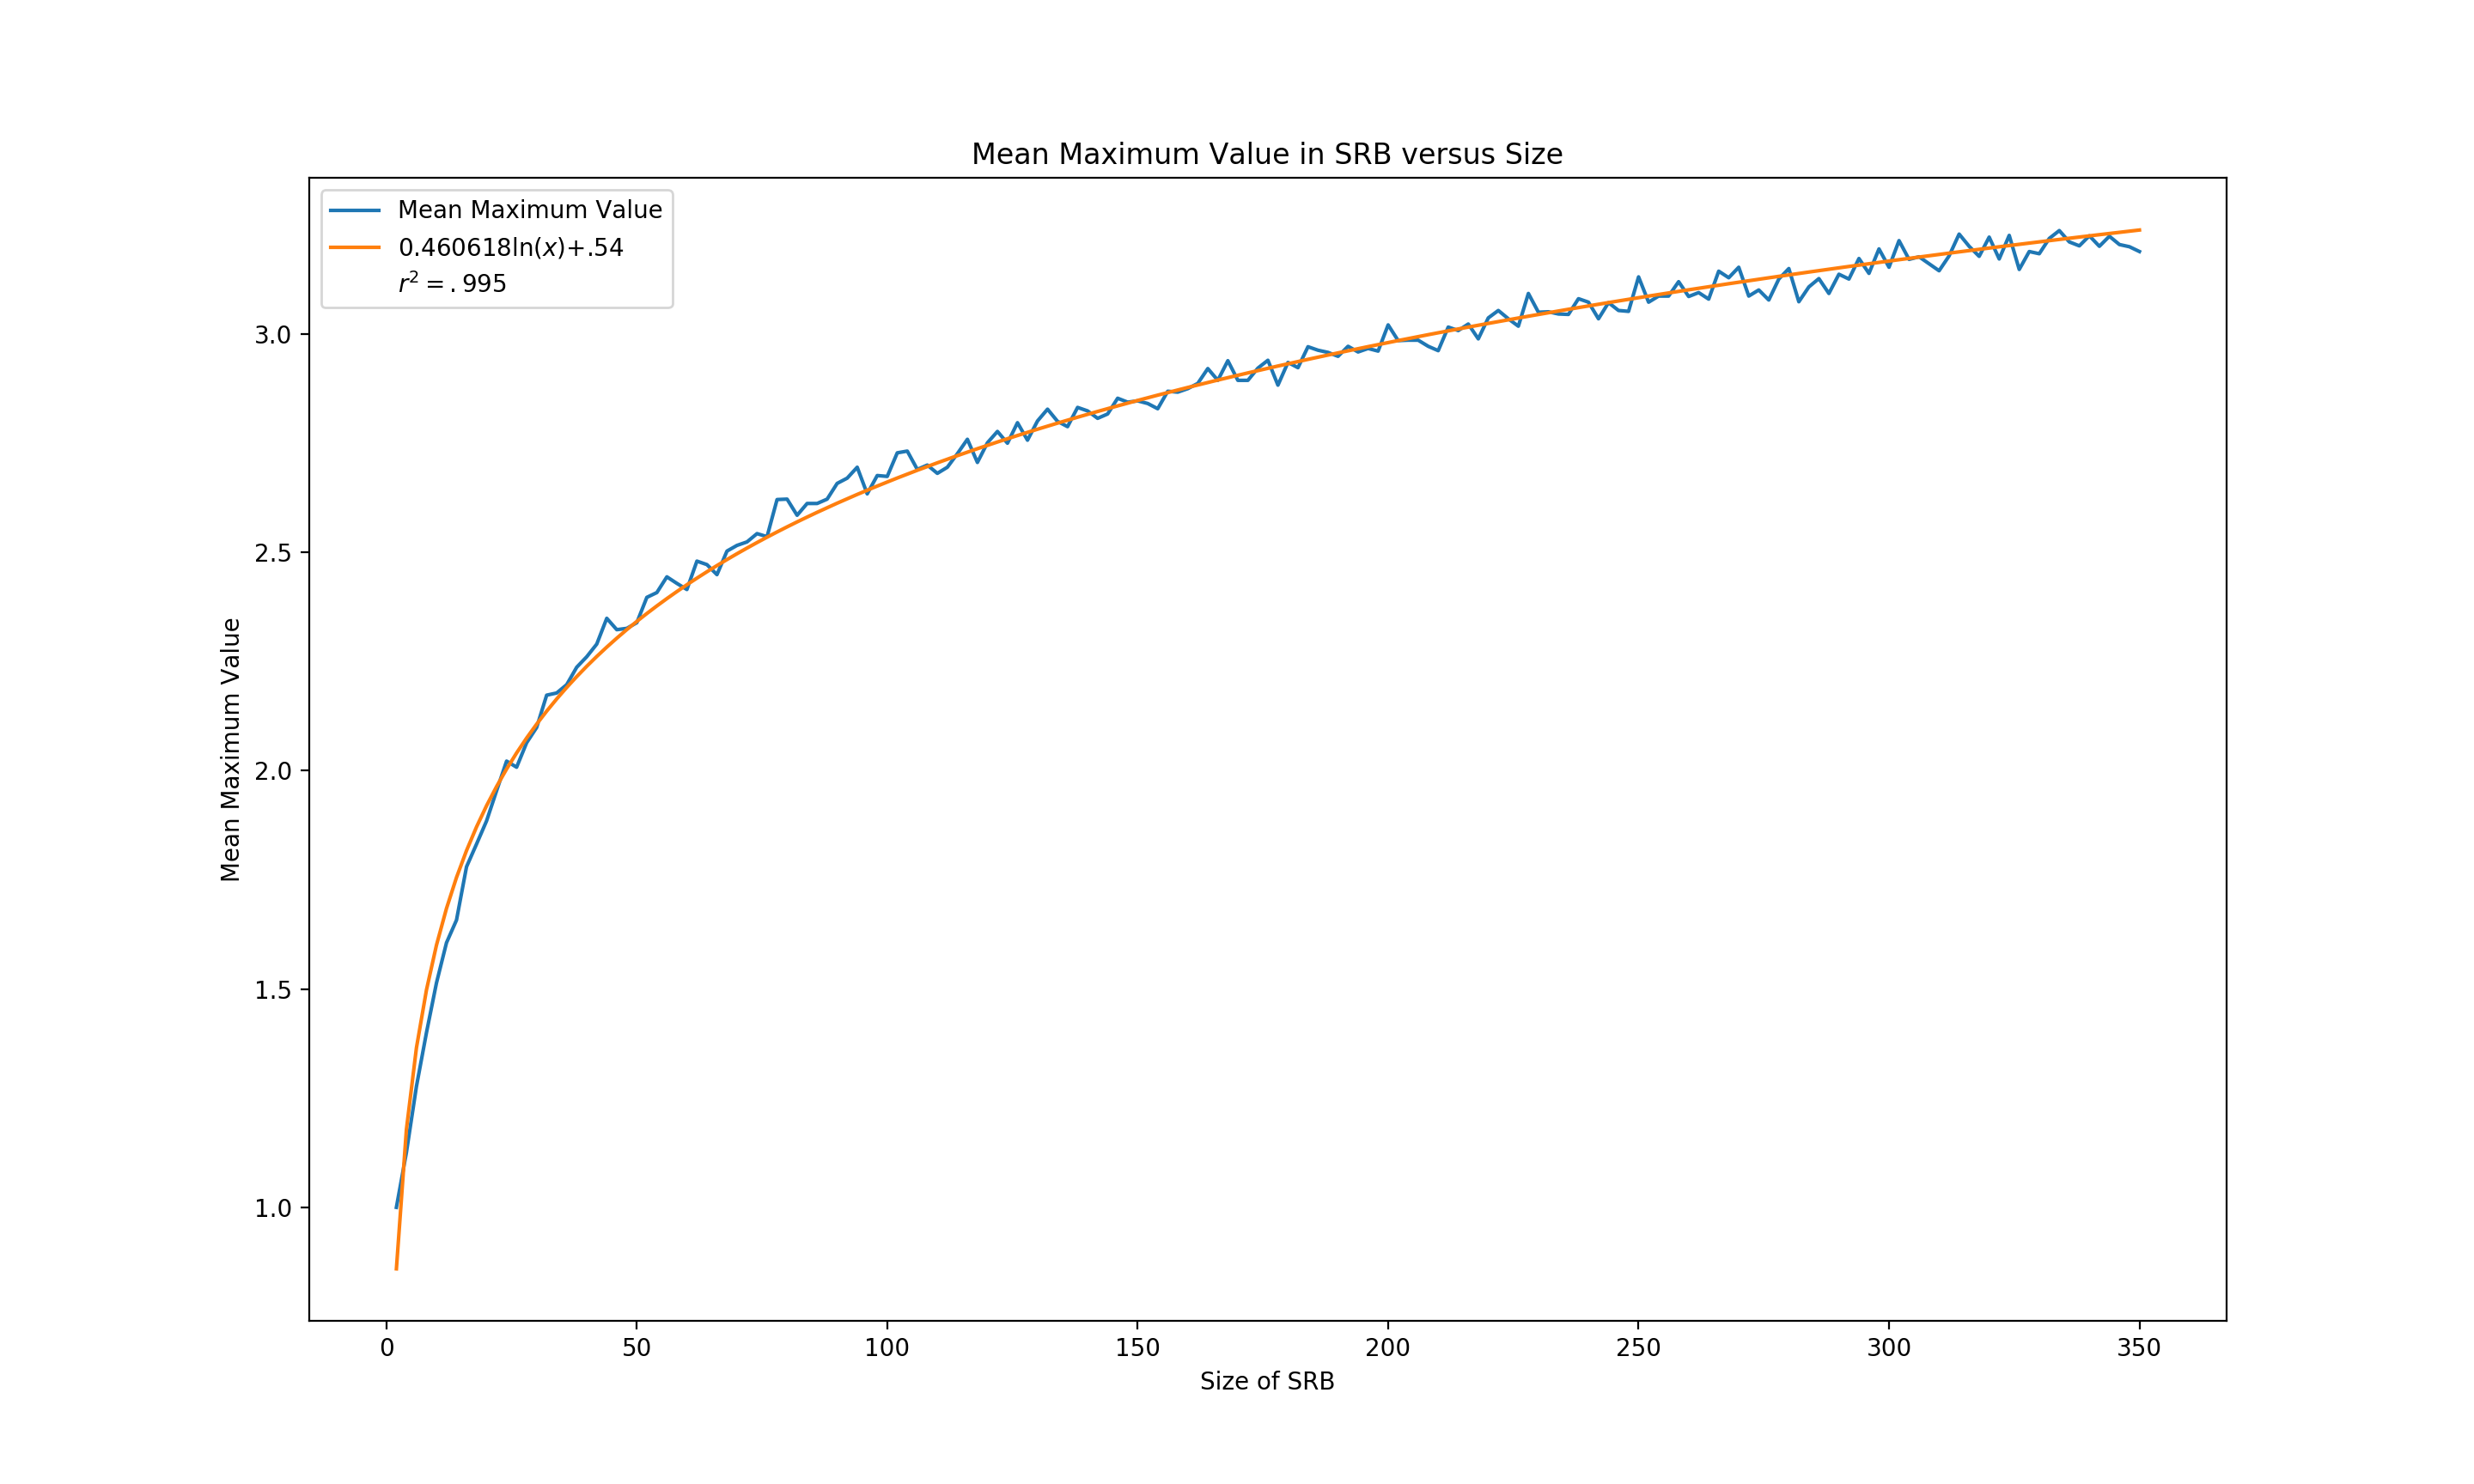
\includegraphics[width=\textwidth]{Figure_4}
\end{figure}


\section{Probability of point specific flips under addition}

One way that one might hope to understand the behavior of SRBs under addition would be to examine the probability that any individual down point is flipped. A specific SRB with its points colored according to the probability that they are flipped is shown in Figure 5. While sharp general results seem hard to come by, there are a few simple statements that one can make about these probabilities.

In the below proposition and throughout, the probability is taken uniformly as $B$ is added with all test bridges $B_0$ of size $N$.

\begin{proposition} Let $B$ be the SRB of size $N$ defined by $B(i):=(i\,\,\mathrm{mod}(2))$, which is well defined as there are no SRBs for which $N$ is odd. It holds that $\Pr[0\,\,\mathrm{flips}]=\frac{2}{N+2}$.
\end{proposition}

\begin{proof} By the definition of probability we have that

$$\Pr[0\,\,\mathrm{flips}]=\frac{|\{B_0 \,\, \mathrm{flips\,\, }0\}|}{|\{B_0\,\,\mathrm{of\,\,size\,\,N}\}|}$$

Since $\sum_i (B(i+1)-B(i))=0$ we have that $B(i+1)-B(i)=1$ and $B(i+1)-B(i)=-1$ exactly $N/2$ times, the placement of the $N/2$ $+1s$ in $B(i+1)-B(i)$ exactly determines the placement of $B(i+1)-B(i)=-1$s. Thus, the total amount of SRBs of size $N$ is ${N \choose N/2}$.

Any bridge $B_0$ that never intersects $B$ will flip $0$ since then $\max(B_0(i)-B(i))=0=B_0(0)-B(0)$. As discussed above any bridge can be determined by the distribution of $+1$s and $-1$s in $B_0(i+1)-B_0(i)$. $B_0$ will not intersect $B$ if and only if the number of $-1s$ in any intial segment of $B_0(i)$s if greater or equal to the number of $+1$s.

These sorts of sequences of $\pm1$s are known as Dyck words, and it is well known that the amount of Dyck words of length $N$ is exactly $\frac{2}{N+2}{N\choose N/2}$ \cite{duchon2000enumeration}
\end{proof}

\begin{figure}[h!]
\caption{An SRB with flip probability coloring}
\centering
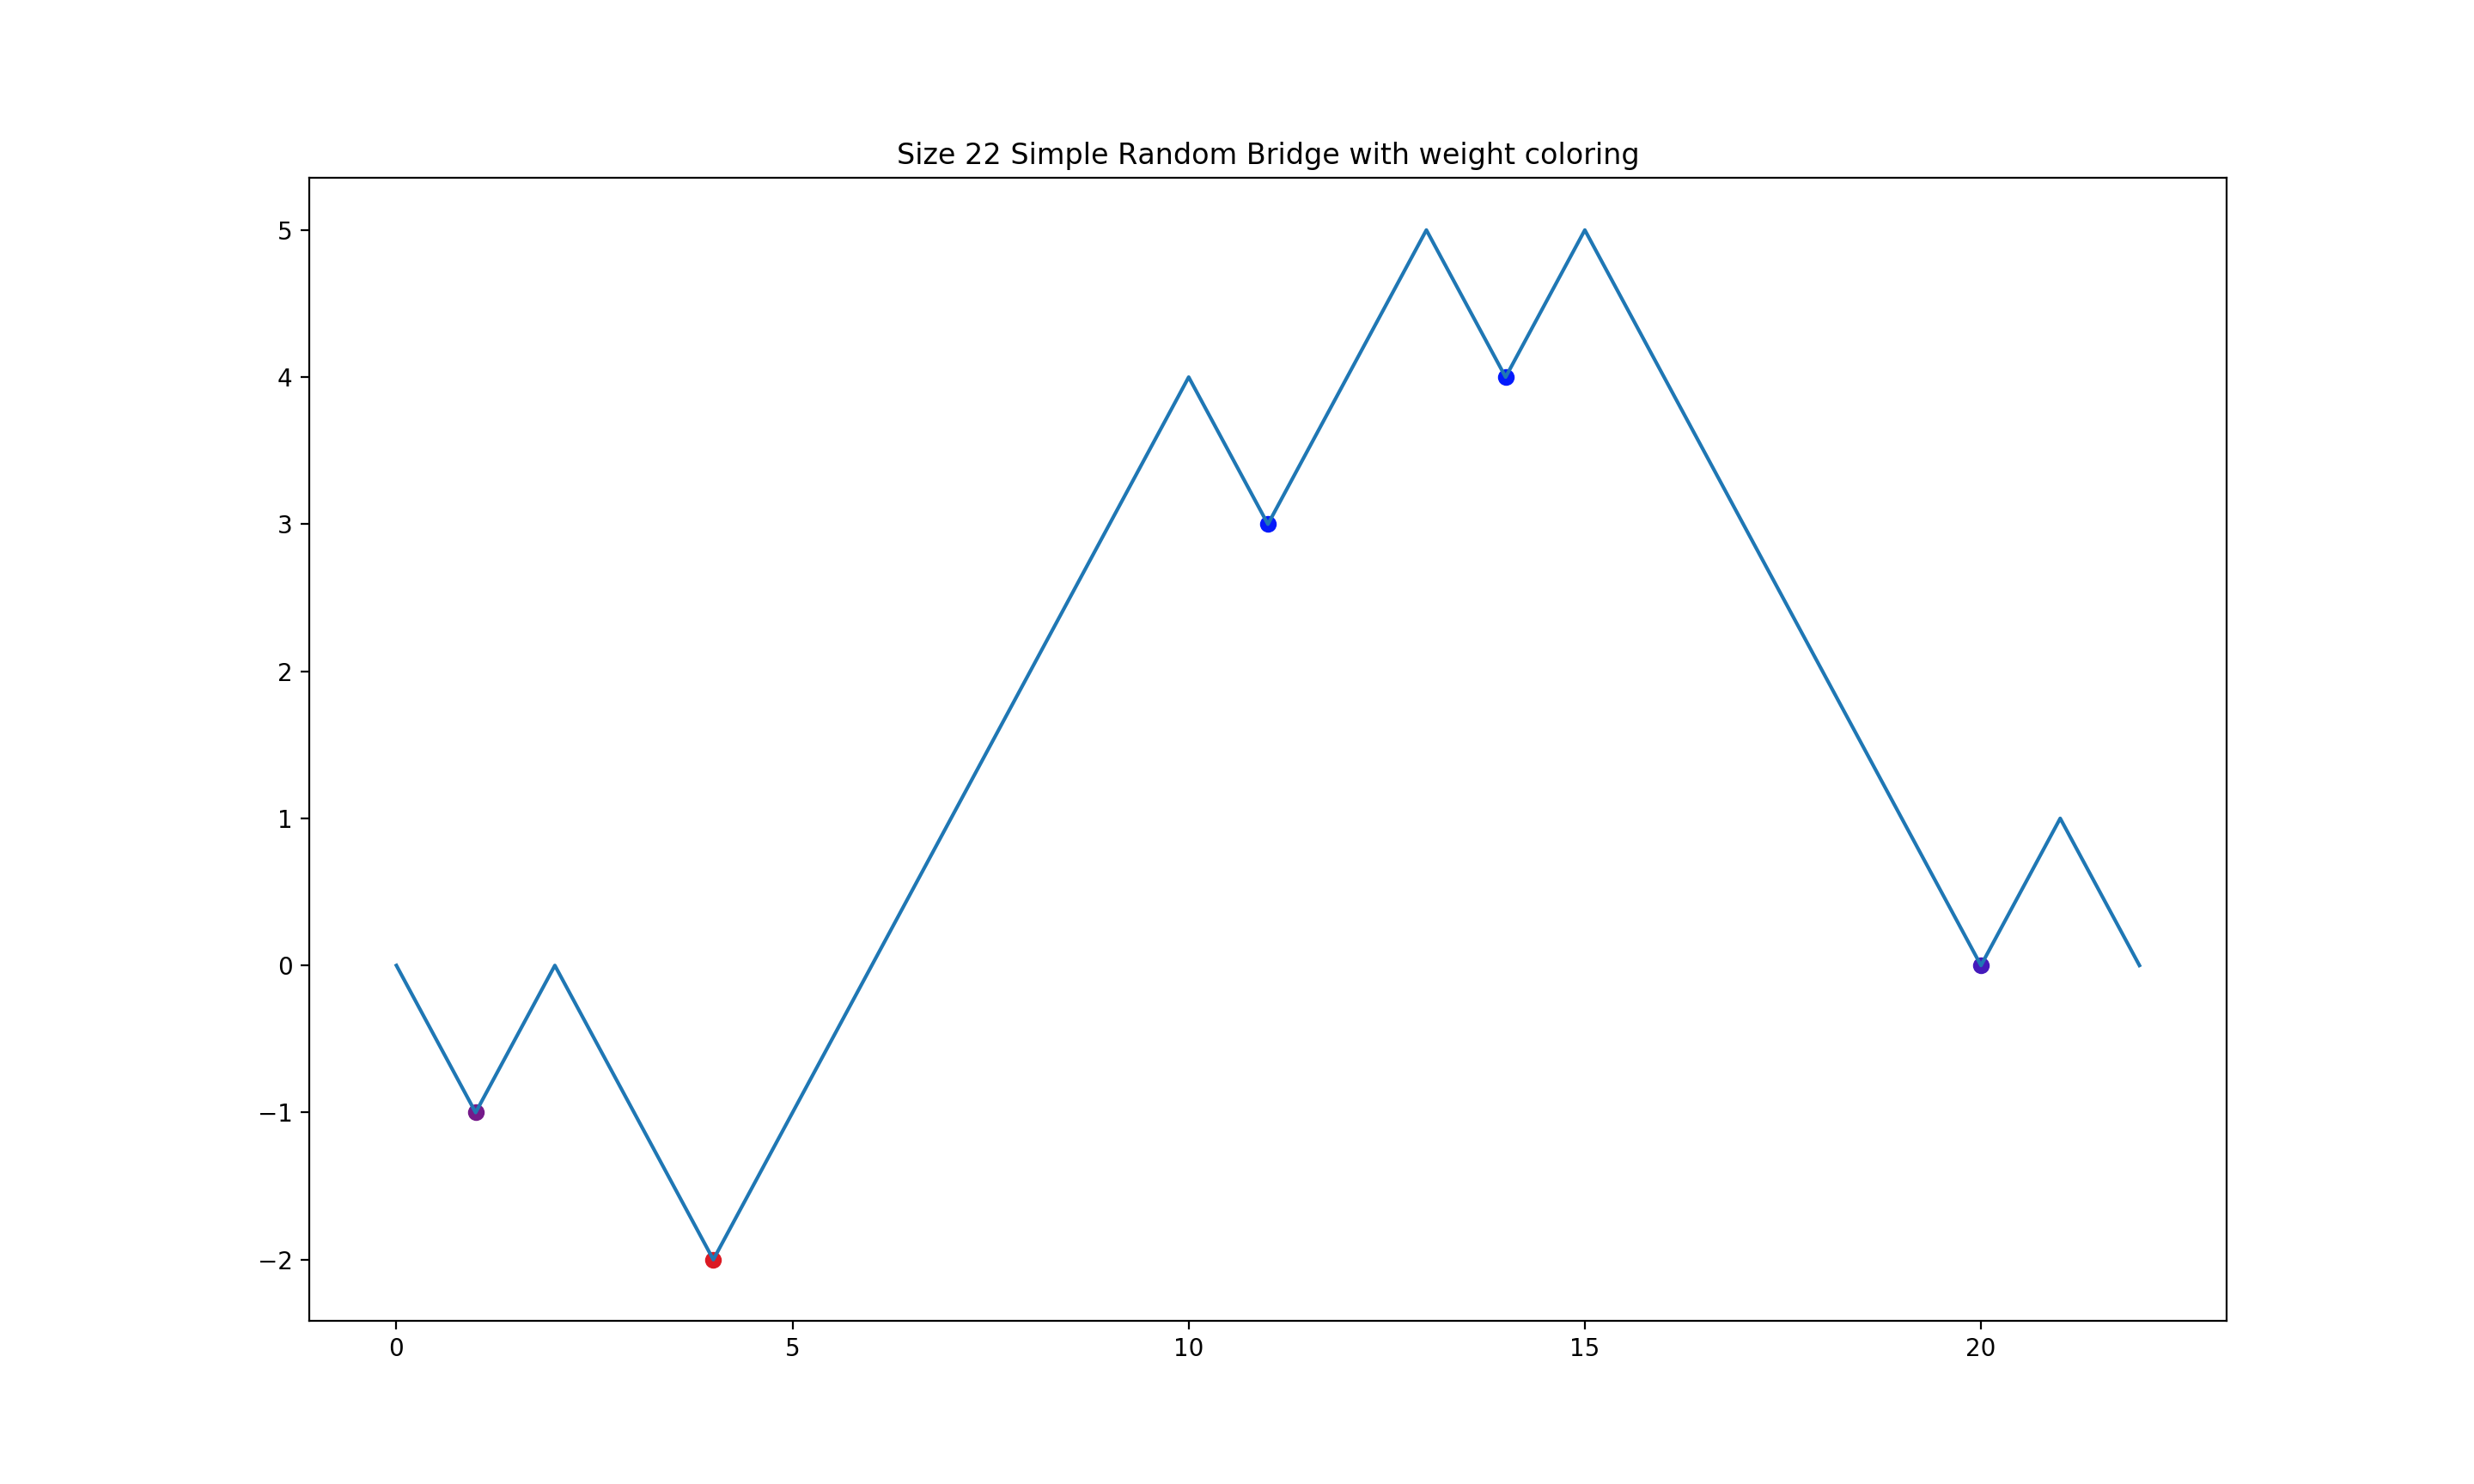
\includegraphics[width=\textwidth]{Figure_5}
\end{figure}

As a simple corollary, we arrive at a general lower bound for how likely a point is to be flipped, if it is (one of) the points the lowest in the image.

\begin{corollary} For any bridge $B$ and index $i$, if $B(i)=\min_jB(j)$ then $\Pr[i \mathrm{\,\, flips}]\geq \frac{2}{N+2}$.
\end{corollary}
\begin{proof} If we define a new Bridge $B'$ by $B'(j):=B(j+i)-B(i)$, then clearly every bridge with the Dyck word property as in the proof of Proposition 1 will once again not intersect $B'$, since by assumtion of minimality we have that $B'(j)\geq0$ uniformly. Thus,

$$|\{B_0 \,\, \mathrm{flips\,\, }i\}|\geq \frac{2}{N+2}{N\choose N/2}$$

and plugging this into

$$\Pr[i\,\,\mathrm{flips}]=\frac{|\{B_0 \,\, \mathrm{flips\,\, }i\}|}{|\{B_0\,\,\mathrm{of\,\,size\,\,N}\}|}$$

we are done.
\end{proof}
\bibliographystyle{plain}
\bibliography{ref}


\end{document}

